\documentclass[11pt,letterpaper]{report}

% ---------------------------------------------------------------
% Paquetes
% ---------------------------------------------------------------
\usepackage[utf8]{inputenc}
\usepackage[T1]{fontenc}
\usepackage[spanish,es-nodecimaldot,es-tabla]{babel}
\usepackage{amsmath,amssymb}
\usepackage{graphicx}
\usepackage{booktabs}
\usepackage{float}
\usepackage[margin=2.5cm]{geometry}
\usepackage{xcolor}
\usepackage{listings}
\usepackage{algorithm}
\usepackage{algpseudocode}
\usepackage{hyperref}
\usepackage{caption}

\graphicspath{{figuras/}}

\lstset{
  language=Python,
  basicstyle=\ttfamily\small,
  keywordstyle=\color{blue},
  commentstyle=\color{gray},
  stringstyle=\color{teal},
  frame=single,
  breaklines=true,
  showstringspaces=false,
  numbers=left,
  numberstyle=\tiny\color{gray}
}

\floatname{algorithm}{Algoritmo}
\renewcommand{\algorithmicrequire}{\textbf{Entrada:}}
\renewcommand{\algorithmicensure}{\textbf{Salida:}}

% Quitar el espacio grande al inicio de cada capítulo
\usepackage{titlesec}
\titleformat{\chapter}[display]
  {\normalfont\huge\bfseries}{\chaptertitlename\ \thechapter}{10pt}{\Huge}
\titlespacing*{\chapter}{0pt}{-30pt}{20pt}

\begin{document}

% ---------------------------------------------------------------
% Portada
% ---------------------------------------------------------------
\begin{titlepage}
\centering
% Logo de la universidad: subir la imagen a Overleaf con el nombre "logo.png"
% (en la misma carpeta que este archivo). Mientras no exista, se muestra un recuadro.
\IfFileExists{logo.png}{%
  \includegraphics[width=5cm]{logo.png}%
}{%
  \fbox{\parbox[c][3cm][c]{5cm}{\centering Logo de la universidad}}%
}\\[1.5cm]

{\LARGE \textbf{Proyecto Final -- Análisis Numérico}}\\[0.6cm]
{\Large Integración adaptativa mediante la regla de Simpson}\\[2.5cm]

{\large \textbf{Integrantes}}\\[0.4cm]
\begin{tabular}{ll}
Juan Diego Acosta Ojeda      & ID: 185015 \\
Sergio Emilio López Montalvo & ID: 186545 \\
\end{tabular}

\vfill
{\large \today}
\end{titlepage}

\tableofcontents

% =================================================================
\chapter{Explicación matemática del método}
% =================================================================

\section{Planteamiento del problema}
Se desea aproximar la integral definida
\[
  I = \int_a^b f(x)\,dx .
\]
Los métodos de integración numérica reemplazan $f$ por un polinomio interpolante
fácil de integrar. La \textbf{regla de Simpson} usa un polinomio de grado 2
(una parábola). La \textbf{integración adaptativa} aplica esta regla en subintervalos
cuyo tamaño se ajusta automáticamente según el comportamiento local de la función.

\section{Fundamento de la regla de Simpson}
Sea $m=\frac{a+b}{2}$ y $h=\frac{b-a}{2}$. Se construye el único polinomio
$p_2(x)$ de grado $\le 2$ que pasa por los puntos $(a,f(a))$, $(m,f(m))$ y $(b,f(b))$.
Usando la forma de Lagrange,
\[
p_2(x)=f(a)\frac{(x-m)(x-b)}{(a-m)(a-b)}+f(m)\frac{(x-a)(x-b)}{(m-a)(m-b)}
      +f(b)\frac{(x-a)(x-m)}{(b-a)(b-m)} .
\]
Integrando cada polinomio base de Lagrange sobre $[a,b]$ se obtienen los pesos
$\frac{h}{3},\frac{4h}{3},\frac{h}{3}$, de donde resulta la regla de Simpson:
\begin{equation}
  S(a,b)=\int_a^b p_2(x)\,dx=\frac{h}{3}\Big[f(a)+4f(m)+f(b)\Big]
        =\frac{b-a}{6}\Big[f(a)+4f(m)+f(b)\Big].
  \label{eq:simpson}
\end{equation}

\paragraph{Error de la regla.} Si $f\in C^4[a,b]$, mediante un desarrollo de Taylor se demuestra que
\begin{equation}
  I-S(a,b)=-\frac{h^5}{90}f^{(4)}(\xi),\qquad \xi\in(a,b).
  \label{eq:error}
\end{equation}
Por lo tanto la regla es exacta para polinomios de grado $\le 3$ y el error local
es de orden $\mathcal{O}(h^5)$.

\paragraph{Simpson compuesto.} Si $[a,b]$ se divide en $n$ (par) subintervalos de ancho
$h=(b-a)/n$, con nodos $x_i=a+ih$,
\begin{equation}
  S_n=\frac{h}{3}\Big[f(x_0)+4\sum_{i\ \text{impar}}f(x_i)+2\sum_{i\ \text{par}}f(x_i)+f(x_n)\Big],
  \qquad I-S_n=-\frac{(b-a)h^4}{180}f^{(4)}(\xi).
\end{equation}
El compuesto usa $n+1$ evaluaciones y su error es $\mathcal{O}(h^4)$, pero con el
\emph{mismo} $h$ en todo el intervalo: si la función es difícil sólo en una pequeña región,
el paso pequeño que esa región necesita se desperdicia en el resto del intervalo.

\section{Estimación del error comparando dos aproximaciones}
En un intervalo $[a,b]$ se calculan dos aproximaciones con distinto tamaño de paso:
\begin{align*}
  S_1 &= S(a,b) && \text{(paso } h\text{)},\\
  S_2 &= S(a,m)+S(m,b) && \text{(paso } h/2\text{)}.
\end{align*}
Por \eqref{eq:error}, suponiendo que $f^{(4)}$ es aproximadamente constante en $[a,b]$:
\[
  I-S_1\approx -\frac{h^5}{90}f^{(4)},\qquad
  I-S_2\approx -2\cdot\frac{(h/2)^5}{90}f^{(4)}=\frac{1}{16}\left(-\frac{h^5}{90}f^{(4)}\right).
\]
Es decir, $I-S_1\approx 16\,(I-S_2)$. Restando:
\[
  S_2-S_1=(I-S_1)-(I-S_2)\approx 15\,(I-S_2)
  \quad\Longrightarrow\quad
  \boxed{\,|I-S_2|\approx E=\frac{|S_2-S_1|}{15}\,}
\]
Así se obtiene una estimación del error \textbf{sin conocer el valor exacto} y sin
necesidad de calcular $f^{(4)}$. Además se puede usar la corrección
(extrapolación de Richardson)
\begin{equation}
  I\approx S_2+\frac{S_2-S_1}{15},
\end{equation}
que elimina el término principal del error (resulta una regla de orden $\mathcal{O}(h^7)$,
la regla de Boole).

\section{Procedimiento de subdivisión recursiva}
\begin{enumerate}
  \item Se calcula $S_1$ en $[a,b]$ y $S_2$ usando sus dos mitades.
  \item Se estima el error $E=|S_2-S_1|/15$.
  \item Si $E$ cumple la tolerancia, el intervalo se \textbf{acepta} y se devuelve
        $S_2+(S_2-S_1)/15$.
  \item Si no, el intervalo se \textbf{divide} en $[a,m]$ y $[m,b]$ y se aplica el
        mismo procedimiento a cada mitad con la mitad de la tolerancia absoluta.
  \item La integral es la suma de los resultados de todos los subintervalos aceptados.
\end{enumerate}
Como las aproximaciones $S(a,m)$ y $S(m,b)$ calculadas en el paso 1 son exactamente
las $S_1$ de los hijos, y los puntos $a,\frac{a+m}{2},m,\frac{m+b}{2},b$ ya fueron
evaluados, cada hijo sólo necesita \textbf{dos evaluaciones nuevas} de $f$.

\section{Criterio de aceptación de un subintervalo}
Un subintervalo $[a_i,b_i]$ que se encuentra en el nivel $k$ de la recursión
(es decir, de longitud $(b-a)/2^k$) se acepta si
\begin{equation}
  \frac{|S_2-S_1|}{15}\ \le\ \max\!\left(\frac{\varepsilon_{\text{abs}}}{2^{k}},\ \varepsilon_{\text{rel}}\,|S_2|\right).
  \label{eq:criterio}
\end{equation}

\section{Papel de las tolerancias absoluta y relativa}
\begin{itemize}
  \item \textbf{Tolerancia absoluta $\varepsilon_{\text{abs}}$:} controla el error en
        las mismas unidades que la integral. Se reparte entre los subintervalos: al dividir
        un intervalo, cada mitad recibe $\varepsilon_{\text{abs}}/2$. Como en el nivel $k$
        hay como máximo $2^k$ intervalos, la suma de los errores locales queda acotada
        aproximadamente por $\varepsilon_{\text{abs}}$.
        Es importante cuando la integral es cercana a cero (por ejemplo $\int_0^2\sin(20x)\,dx\approx 0.083$),
        caso en el que un criterio puramente relativo sería demasiado exigente.
  \item \textbf{Tolerancia relativa $\varepsilon_{\text{rel}}$:} pide un número de cifras
        significativas correctas, independientemente de la escala de $f$. Si la integral es
        muy grande, exigir un error absoluto pequeño sería innecesario (o imposible por el
        redondeo); la parte relativa evita ese esfuerzo inútil.
  \item Al tomar el \textbf{máximo} de ambas, el intervalo se acepta en cuanto se cumple
        cualquiera de los dos requisitos, que es el mismo criterio que usan bibliotecas
        como \texttt{scipy.integrate.quad}.
\end{itemize}

\section{Límite de profundidad}
Para garantizar que el algoritmo termine (por ejemplo, si $f$ tiene una singularidad o si
el error de redondeo impide alcanzar la tolerancia), se impone una profundidad máxima
$k_{\max}$. Si un intervalo llega a esa profundidad se acepta aunque no cumpla
\eqref{eq:criterio} y se registra como \emph{no convergido}.

% =================================================================
\chapter{Implementación computacional}
% =================================================================

\section{Organización del código}
El código se escribió desde cero en Python, usando sólo la biblioteca estándar para el
algoritmo. NumPy y Matplotlib se usan para las gráficas, y \texttt{scipy.integrate.quad}
se usa \textbf{únicamente como referencia} en los experimentos.
\begin{itemize}
  \item \texttt{simpson\_adaptativo.py}: funciones \texttt{simpson\_simple},
        \texttt{simpson\_compuesto} y \texttt{simpson\_adaptativo}.
  \item \texttt{experimentos.py}: ejecuta todos los experimentos y guarda las tablas
        (\texttt{resultados/*.csv}) y las figuras (\texttt{figuras/*.png}).
\end{itemize}

\section{Algoritmo}
\begin{algorithm}[H]
\caption{Simpson adaptativo}
\begin{algorithmic}[1]
\Require $f$, $a$, $b$, $\varepsilon_{\text{abs}}$, $\varepsilon_{\text{rel}}$, $k_{\max}$
\Ensure aproximación de $I$, número de evaluaciones, lista de subintervalos
\State $f_a\gets f(a)$, $f_b\gets f(b)$, $f_m\gets f(\frac{a+b}{2})$ \Comment{3 evaluaciones}
\State $S_1\gets \frac{b-a}{6}(f_a+4f_m+f_b)$
\State \Return \Call{Paso}{$a,b,f_a,f_m,f_b,S_1,\varepsilon_{\text{abs}},0$}
\Statex
\Function{Paso}{$a,b,f_a,f_m,f_b,S_1,\tau,k$}
  \State $m\gets\frac{a+b}{2}$;\quad $f_{l}\gets f(\frac{a+m}{2})$;\quad $f_{r}\gets f(\frac{m+b}{2})$ \Comment{2 evaluaciones nuevas}
  \State $S_{izq}\gets S(a,m)$,\quad $S_{der}\gets S(m,b)$,\quad $S_2\gets S_{izq}+S_{der}$
  \State $E\gets |S_2-S_1|/15$
  \If{$E\le\max(\tau,\ \varepsilon_{\text{rel}}|S_2|)$ \textbf{or} $k\ge k_{\max}$}
     \State guardar $[a,b]$ en la lista de subintervalos
     \State \Return $S_2+(S_2-S_1)/15$
  \EndIf
  \State \Return \Call{Paso}{$a,m,f_a,f_l,f_m,S_{izq},\tau/2,k+1$} $+$ \Call{Paso}{$m,b,f_m,f_r,f_b,S_{der},\tau/2,k+1$}
\EndFunction
\end{algorithmic}
\end{algorithm}

\section{Código principal}
El núcleo del método es la función recursiva interna (extracto de
\texttt{simpson\_adaptativo.py}):
\begin{lstlisting}
def paso_recursivo(a, b, fa, fm, fb, S1, tol_a, prof):
    m = (a + b) / 2.0
    ml = (a + m) / 2.0
    mr = (m + b) / 2.0
    fml = evaluar(ml)        # unicas evaluaciones nuevas
    fmr = evaluar(mr)

    S_izq = simpson_simple(a, m, fa, fml, fm)
    S_der = simpson_simple(m, b, fm, fmr, fb)
    S2 = S_izq + S_der

    error = abs(S2 - S1) / 15.0
    tolerancia = max(tol_a, tol_rel * abs(S2))

    if error <= tolerancia or prof >= max_prof:
        if error > tolerancia:
            info["sin_converger"] += 1
        info["intervalos"].append((a, b))
        info["error_estimado"] += error
        return S2 + (S2 - S1) / 15.0

    izquierda = paso_recursivo(a, m, fa, fml, fm, S_izq, tol_a / 2.0, prof + 1)
    derecha   = paso_recursivo(m, b, fm, fmr, fb, S_der, tol_a / 2.0, prof + 1)
    return izquierda + derecha
\end{lstlisting}

\section{Cumplimiento de los requisitos}
\begin{table}[H]
\centering
\begin{tabular}{p{6cm}p{8.5cm}}
\toprule
\textbf{Requisito} & \textbf{Cómo se cumple} \\
\midrule
Intervalos arbitrarios $[a,b]$ & $a$ y $b$ son parámetros; todos los puntos se calculan a partir de ellos. \\
Estimación local del error & $E=|S_2-S_1|/15$ en cada subintervalo. \\
Tolerancias absoluta y relativa & Parámetros \texttt{tol\_abs} y \texttt{tol\_rel}, criterio \eqref{eq:criterio}. \\
Límite de subdivisiones & Parámetro \texttt{max\_prof} (por defecto 50); se cuentan los intervalos no convergidos. \\
Reutilizar evaluaciones & $f_a,f_m,f_b$ y $S_1$ se pasan al hijo; sólo 2 evaluaciones nuevas por intervalo. \\
Contar evaluaciones & La función interna \texttt{evaluar(x)} incrementa un contador en cada llamada a $f$. \\
Registrar subintervalos & Cada intervalo aceptado se guarda en la lista \texttt{intervalos} del diccionario \texttt{info}. \\
\bottomrule
\end{tabular}
\caption{Requisitos de la implementación.}
\end{table}

\paragraph{Costo.} Si el algoritmo termina con $N$ subintervalos aceptados, el árbol de
recursión tiene $N-1$ intervalos rechazados y $2N-1$ nodos en total. Cada nodo usa 2
evaluaciones nuevas y hay 3 iniciales, por lo que
\[
\text{evaluaciones}=3+2(2N-1)=4N+1 .
\]
Esto se comprueba en todos los experimentos (por ejemplo, $N=104\Rightarrow 417$ evaluaciones
para $I_0$). Sin reutilizar valores, cada nodo necesitaría 5 evaluaciones, es decir
$5(2N-1)\approx 10N$: la reutilización reduce el costo a menos de la mitad.

\paragraph{Valor devuelto.} La función devuelve un diccionario con la integral, el error
estimado (suma de los errores locales), el número de evaluaciones, la lista de subintervalos,
la profundidad máxima alcanzada y el número de intervalos no convergidos.

% =================================================================
\chapter{Experimentación numérica}
% =================================================================

\section{Integrales de prueba}
\begin{table}[H]
\centering
\resizebox{\textwidth}{!}{%
\begin{tabular}{llll}
\toprule
 & \textbf{Integral} & \textbf{Comportamiento} & \textbf{Valor exacto / referencia} \\
\midrule
$I_0$ & $\int_0^4 (x+1)^2\cos\!\left(\frac{2x+1}{x-4.3}\right)dx$ & oscila más rápido cerca de $x=4$ & $-2.825533373437446^{*}$ \\
$I_1$ & $\int_0^1 e^x\,dx$ & suave & $e-1$ \\
$I_2$ & $\int_0^2 \sin(20x)\,dx$ & oscilatoria & $(1-\cos 40)/20$ \\
$I_3$ & $\int_0^1 e^{-100(x-0.5)^2}dx$ & variación localizada & $\frac{\sqrt{\pi}}{10}\operatorname{erf}(5)$ \\
$I_4$ & $\int_0^1 \sqrt{x}\,dx$ & derivadas no acotadas en $x=0$ & $2/3$ \\
\bottomrule
\end{tabular}}
\caption{Integrales estudiadas. $^{*}I_0$ no tiene primitiva elemental: el valor de referencia
se obtuvo con \texttt{scipy.integrate.quad} con tolerancia $10^{-14}$ y coincide con
Simpson adaptativo con $\varepsilon=10^{-10}$ hasta $2\times10^{-13}$.}
\end{table}

La integral $I_0$ corresponde al ejemplo visto en clase (diapositiva 15, clase 25).
La Figura~\ref{fig:funciones} muestra las cinco funciones.

\begin{figure}[H]
\centering
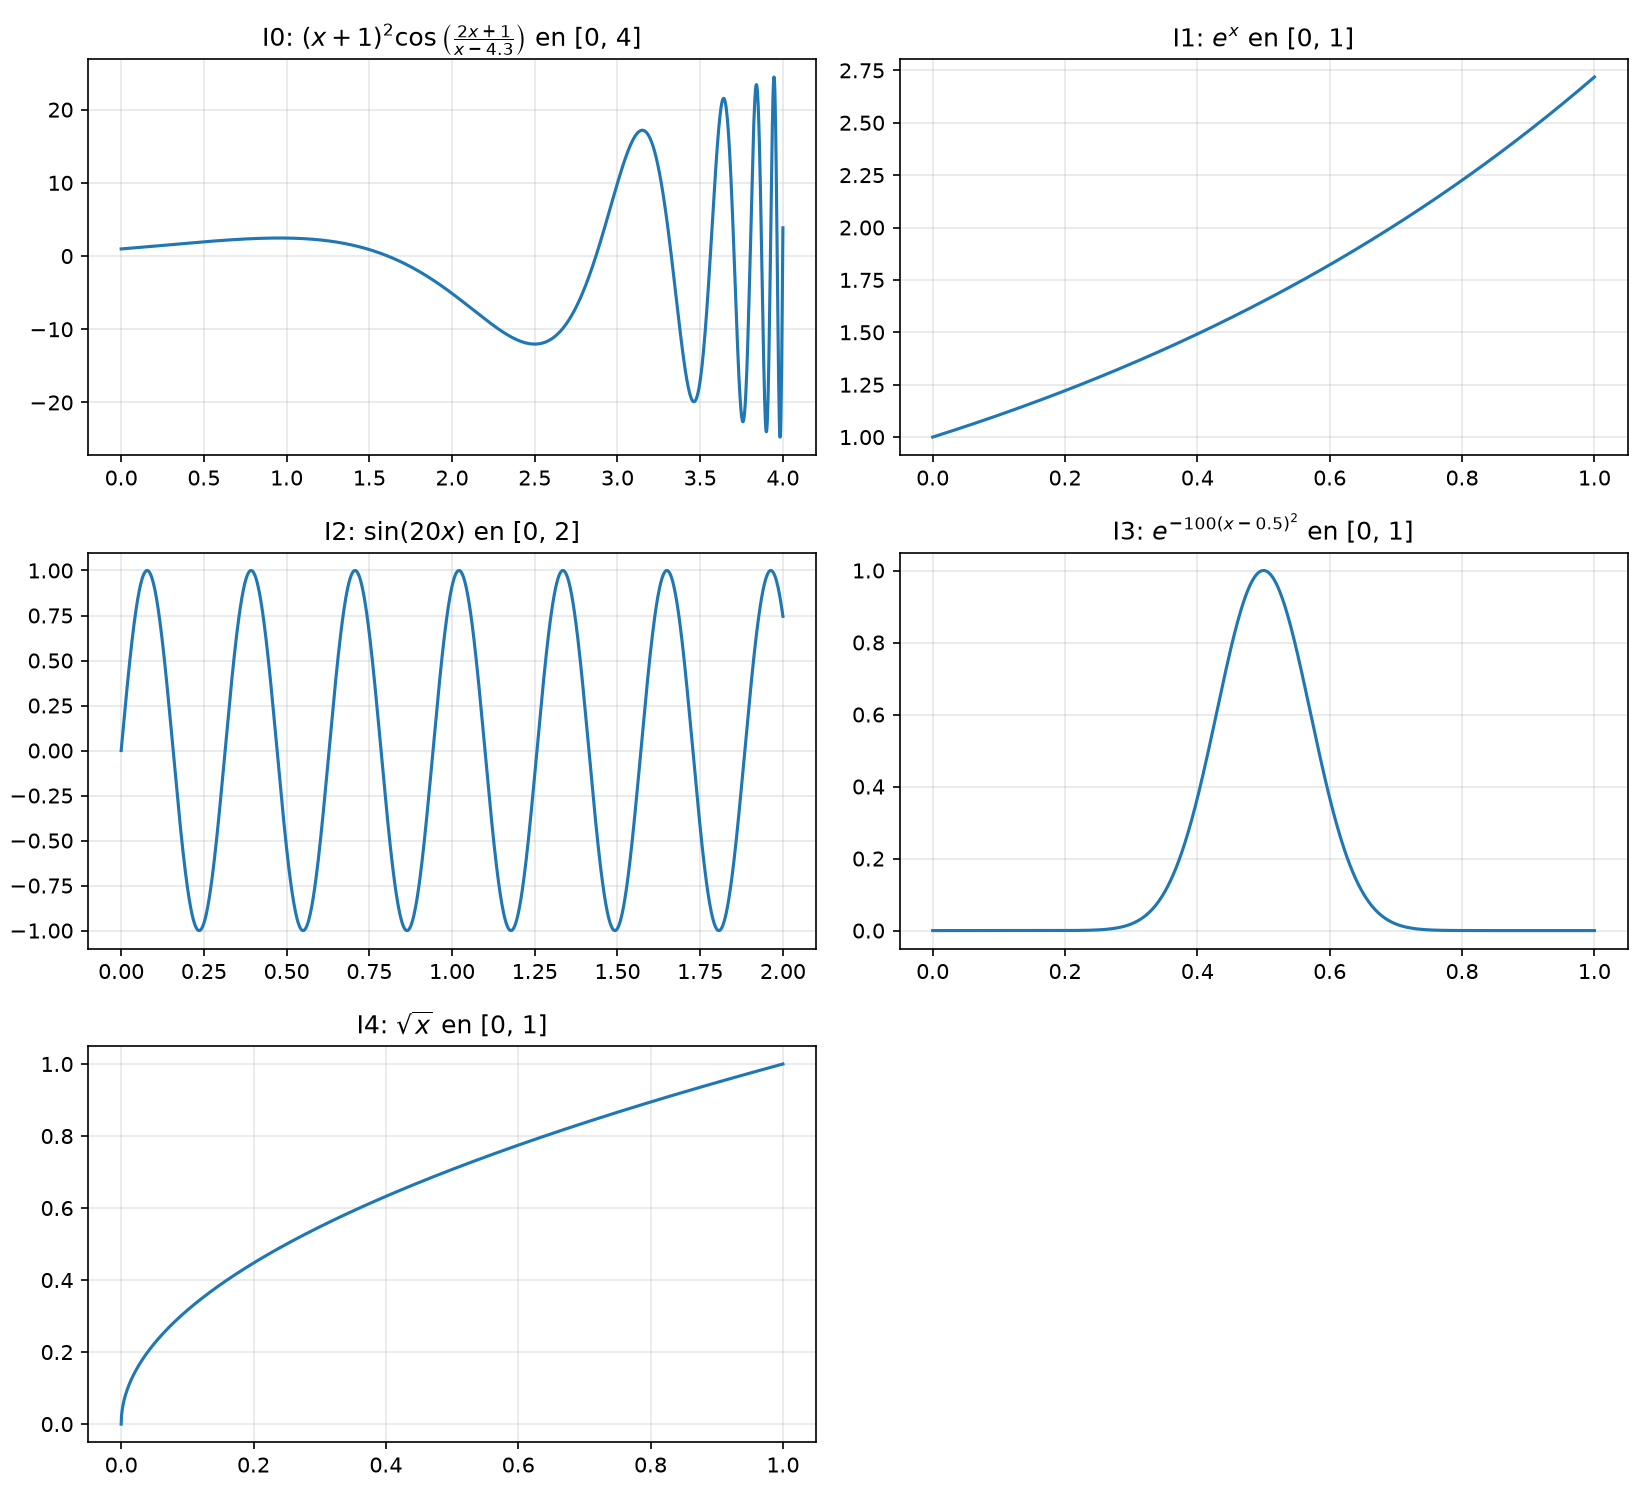
\includegraphics[width=0.9\textwidth]{funciones.png}
\caption{Las cinco funciones integradas.}
\label{fig:funciones}
\end{figure}

\section{Metodología}
\begin{itemize}
  \item Se usó la misma tolerancia para la parte absoluta y la relativa:
        $\varepsilon_{\text{abs}}=\varepsilon_{\text{rel}}=\varepsilon$, con
        $\varepsilon\in\{10^{-2},10^{-3},\dots,10^{-10}\}$ y $k_{\max}=50$.
  \item Para cada caso se registró: el error real $|I-\hat I|$, el error estimado por el
        algoritmo, el número de evaluaciones de $f$, el número de subintervalos y la
        profundidad máxima.
  \item \textbf{Simpson compuesto} se comparó de dos formas: (a) usando el mismo número de
        evaluaciones que el adaptativo, y (b) buscando el menor $n$ con el que alcanza el
        mismo error que el adaptativo (duplicando $n$ y luego por bisección).
  \item \textbf{\texttt{scipy.integrate.quad}} se ejecutó con las mismas tolerancias,
        registrando su error y su número de evaluaciones (\texttt{neval}).
  \item Todos los experimentos son deterministas y se reproducen con
        \texttt{python experimentos.py}.
\end{itemize}

\section{Resultados con tolerancia $\varepsilon=10^{-6}$}
\begin{table}[H]
\centering
\resizebox{\textwidth}{!}{%
\begin{tabular}{lcccccccc}
\toprule
 & \multicolumn{4}{c}{\textbf{Simpson adaptativo}} & \multicolumn{2}{c}{\textbf{Compuesto}} & \multicolumn{2}{c}{\textbf{quad}} \\
\cmidrule(lr){2-5}\cmidrule(lr){6-7}\cmidrule(lr){8-9}
 & error real & error est. & eval. & subint. & error (mismas eval.) & eval. p/ mismo error & error & eval. \\
\midrule
$I_0$ & $5.7\times10^{-8}$  & $9.9\times10^{-6}$ & 417 & 104 & $1.6\times10^{-3}$  & 5275  & $6.7\times10^{-15}$ & 231 \\
$I_1$ & $2.2\times10^{-10}$ & $1.5\times10^{-7}$ & 17  & 4   & $1.5\times10^{-7}$  & 83    & $2.2\times10^{-16}$ & 21 \\
$I_2$ & $1.6\times10^{-10}$ & $3.0\times10^{-7}$ & 501 & 125 & $1.9\times10^{-8}$  & 1645  & $9.7\times10^{-17}$ & 147 \\
$I_3$ & $1.2\times10^{-8}$  & $2.2\times10^{-7}$ & 113 & 28  & $8.6\times10^{-16}$ & 27    & $1.2\times10^{-15}$ & 63 \\
$I_4$ & $2.0\times10^{-8}$  & $2.6\times10^{-7}$ & 105 & 26  & $7.7\times10^{-5}$  & 25849 & $2.2\times10^{-16}$ & 231 \\
\bottomrule
\end{tabular}}
\caption{Comparación de los tres métodos con $\varepsilon=10^{-6}$.}
\label{tab:resumen}
\end{table}

\section{Efecto de la tolerancia}
\begin{table}[H]
\centering
\resizebox{\textwidth}{!}{%
\begin{tabular}{c|rr|rr|rr|rr|rr}
\toprule
 & \multicolumn{2}{c|}{$I_0$} & \multicolumn{2}{c|}{$I_1$} & \multicolumn{2}{c|}{$I_2$} & \multicolumn{2}{c|}{$I_3$} & \multicolumn{2}{c}{$I_4$} \\
$\varepsilon$ & error & eval & error & eval & error & eval & error & eval & error & eval \\
\midrule
$10^{-2}$  & 2.3e-2 & 45   & 8.6e-7  & 5   & 4.1e-4  & 57   & 2.5e-2 & 9   & 8.9e-3  & 5 \\
$10^{-3}$  & 1.3e-4 & 101  & 8.6e-7  & 5   & 1.8e-5  & 101  & 2.5e-2 & 9   & 3.2e-3  & 9 \\
$10^{-4}$  & 2.0e-4 & 149  & 8.6e-7  & 5   & 3.2e-7  & 125  & 3.3e-6 & 33  & 2.7e-6  & 37 \\
$10^{-5}$  & 1.9e-6 & 245  & 1.4e-8  & 9   & 2.0e-8  & 245  & 1.3e-5 & 57  & 5.2e-7  & 61 \\
$10^{-6}$  & 5.7e-8 & 417  & 2.2e-10 & 17  & 1.6e-10 & 501  & 1.2e-8 & 113 & 2.0e-8  & 105 \\
$10^{-7}$  & 3.5e-8 & 773  & 2.2e-10 & 17  & 2.6e-12 & 953  & 2.9e-9 & 177 & 8.0e-10 & 185 \\
$10^{-8}$  & 3.4e-8 & 1377 & 3.4e-12 & 33  & 1.2e-13 & 1785 & 1.3e-9 & 297 & 2.6e-11 & 317 \\
$10^{-9}$  & 1.7e-12& 2533 & 5.3e-14 & 65  & 1.2e-14 & 2025 & 5.1e-11& 553 & 1.0e-12 & 557 \\
$10^{-10}$ & 2.0e-13& 4569 & 6.7e-16 & 129 & 1.8e-16 & 4021 & 8.0e-13& 993 & 2.8e-14 & 985 \\
\bottomrule
\end{tabular}}
\caption{Error real y número de evaluaciones de Simpson adaptativo para cada tolerancia.
La tabla completa (con error estimado, profundidad y comparación con los otros métodos)
está en \texttt{resultados/tabla\_tolerancias.csv}.}
\label{tab:tolerancias}
\end{table}

Para $I_4$ la profundidad máxima creció de 0 ($\varepsilon=10^{-2}$) a 48 ($\varepsilon=10^{-10}$),
muy cerca del límite $k_{\max}=50$; para las demás integrales no pasó de 15.
En ningún experimento se alcanzó el límite de profundidad (0 intervalos no convergidos).

\begin{figure}[H]
\centering
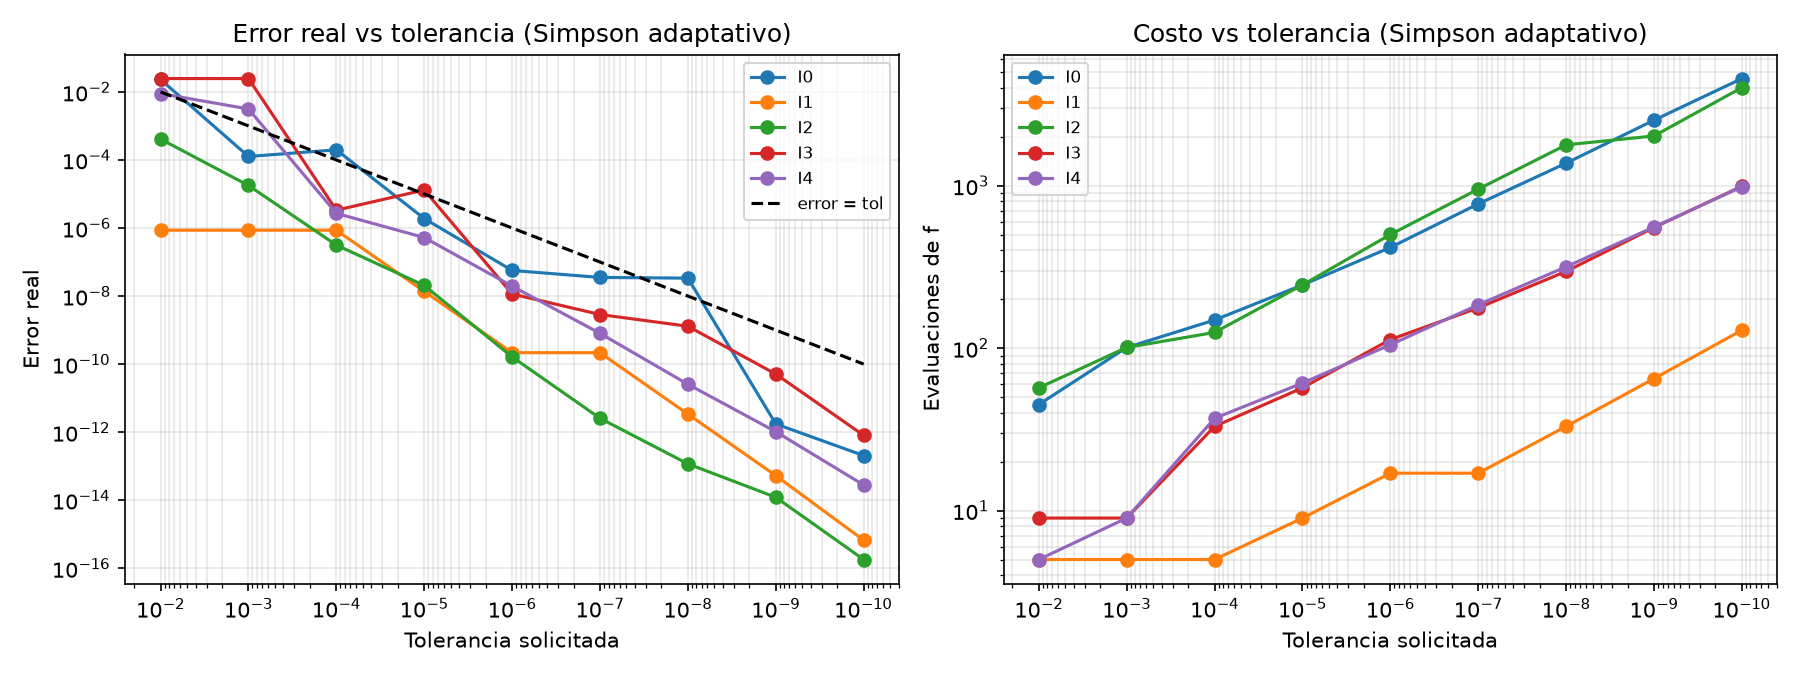
\includegraphics[width=\textwidth]{tolerancia_error_costo.png}
\caption{Izquierda: error real frente a la tolerancia solicitada (la línea discontinua es
error $=$ tolerancia). Derecha: número de evaluaciones frente a la tolerancia.}
\label{fig:tol}
\end{figure}

\section{Error en función del número de evaluaciones}
\begin{figure}[H]
\centering
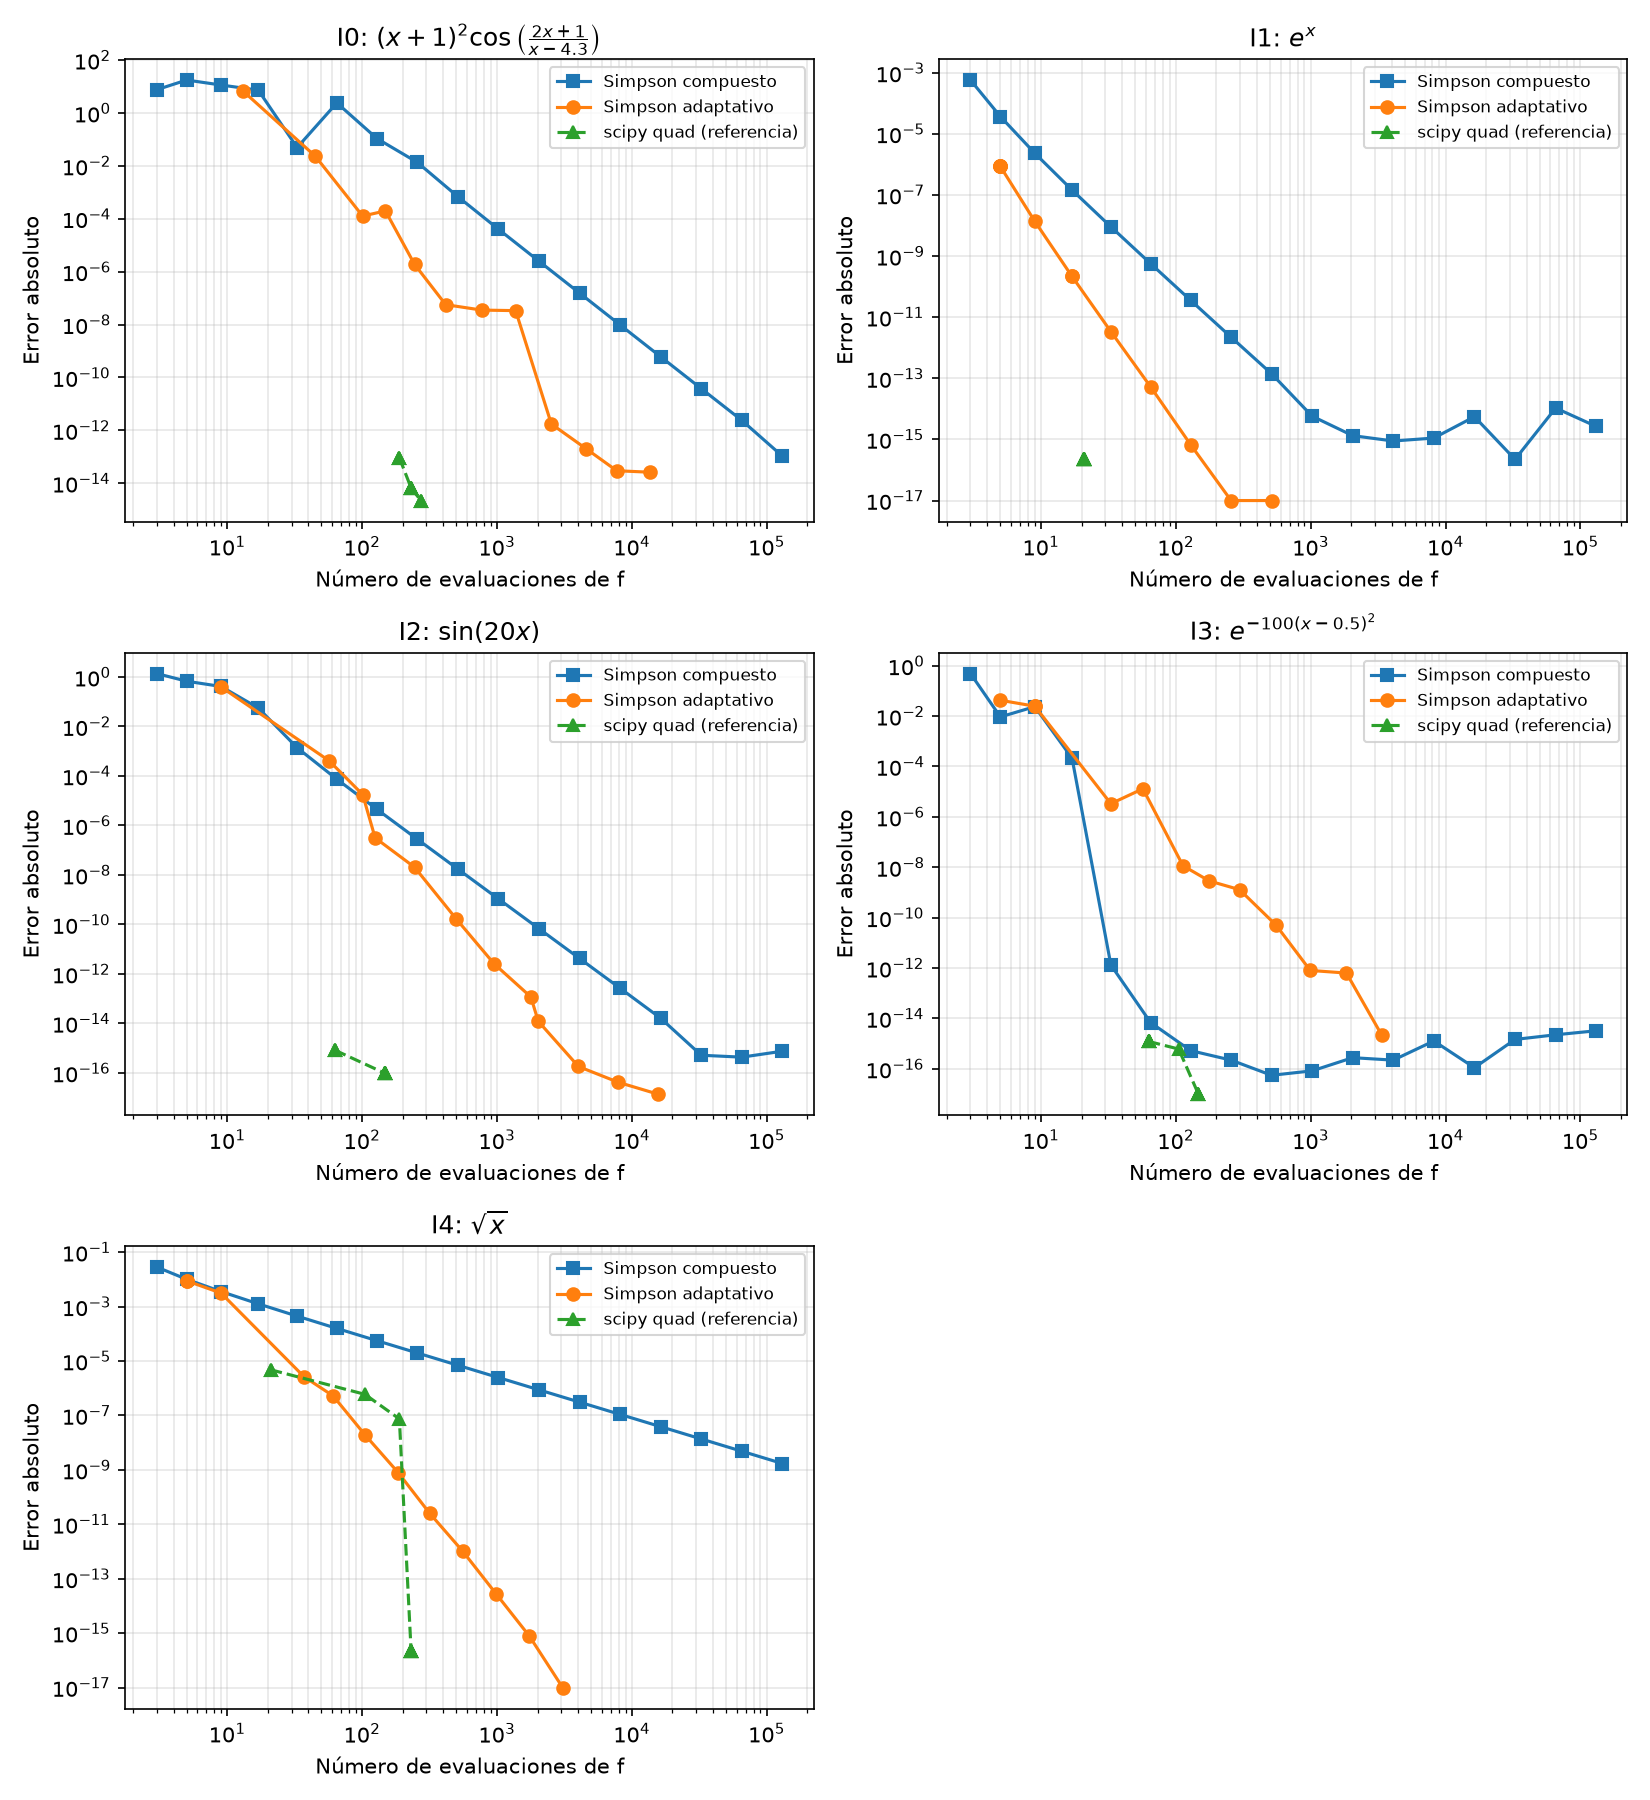
\includegraphics[width=\textwidth]{error_vs_evaluaciones.png}
\caption{Error absoluto frente al número de evaluaciones de $f$ (escala log-log) para
Simpson compuesto ($n=2,4,\dots,2^{17}$), Simpson adaptativo ($\varepsilon=10^{-1},\dots,10^{-12}$)
y \texttt{quad}. Cuanto más abajo y a la izquierda, más eficiente es el método.}
\label{fig:eficiencia}
\end{figure}

\section{Distribución de los subintervalos}
Las Figuras~\ref{fig:sub0}--\ref{fig:sub4} muestran cada función con los bordes de los
subintervalos finales generados por Simpson adaptativo con $\varepsilon=10^{-6}$
(líneas y puntos rojos). En el panel inferior se grafica el ancho $h$ de cada subintervalo
(escala logarítmica) en función de su posición.

\begin{figure}[H]
\centering
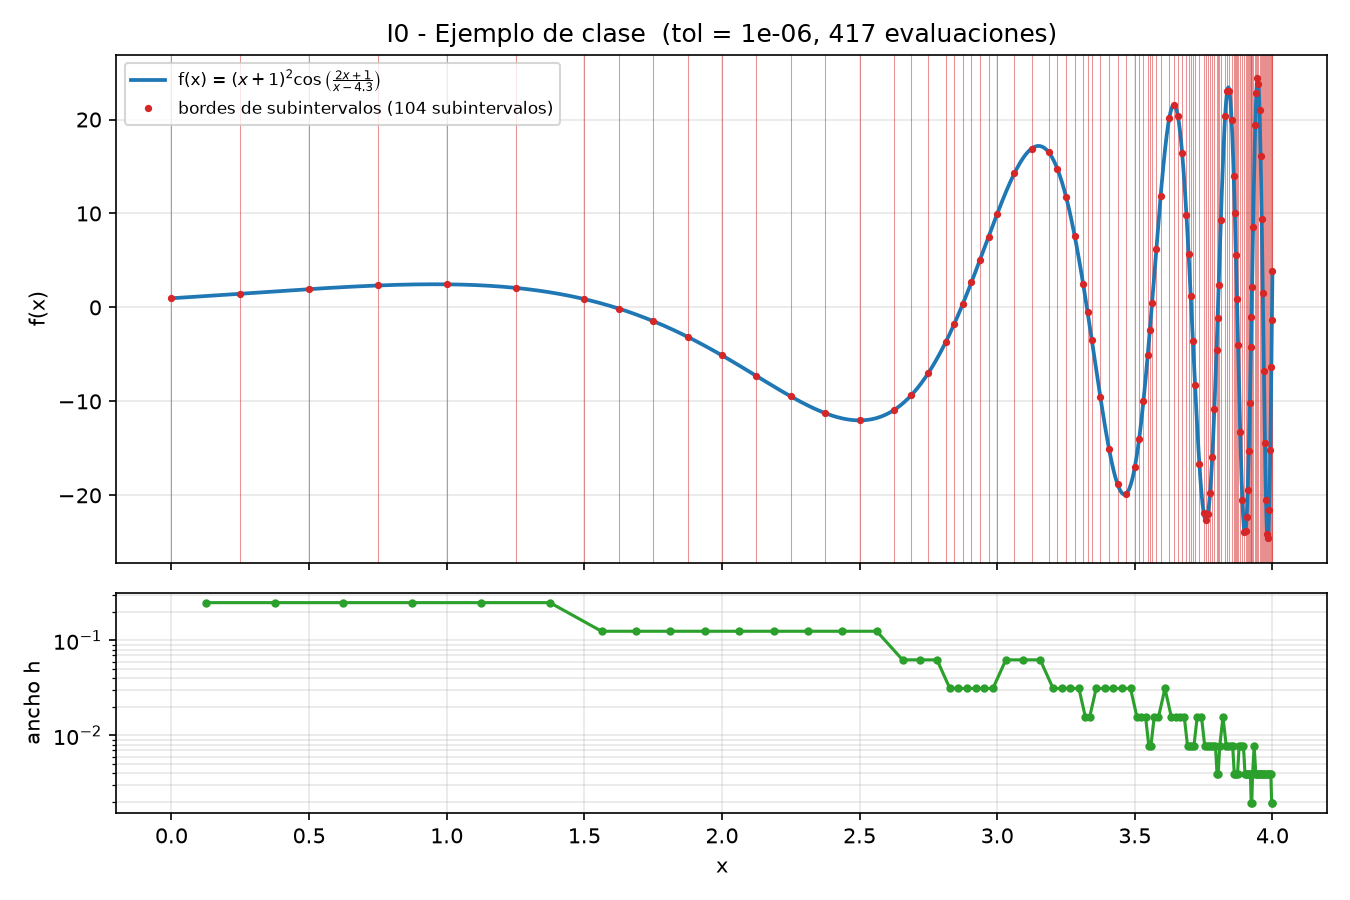
\includegraphics[width=0.85\textwidth]{subintervalos_I0.png}
\caption{$I_0$: los subintervalos se hacen cada vez más pequeños hacia $x=4$.}
\label{fig:sub0}
\end{figure}

\begin{figure}[H]
\centering
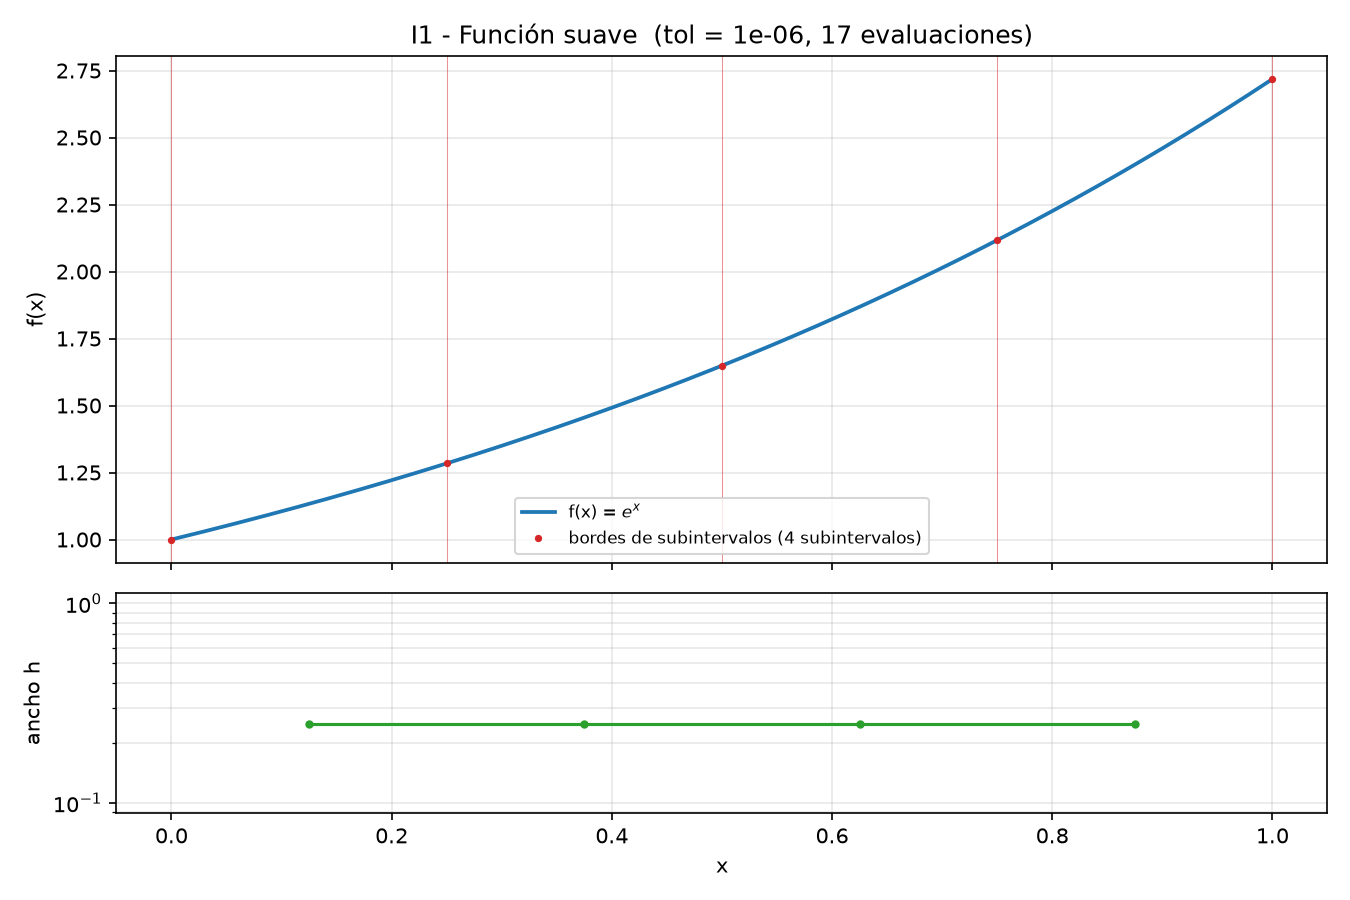
\includegraphics[width=0.85\textwidth]{subintervalos_I1.png}
\caption{$I_1$: función suave, pocos subintervalos y todos del mismo tamaño.}
\label{fig:sub1}
\end{figure}

\begin{figure}[H]
\centering
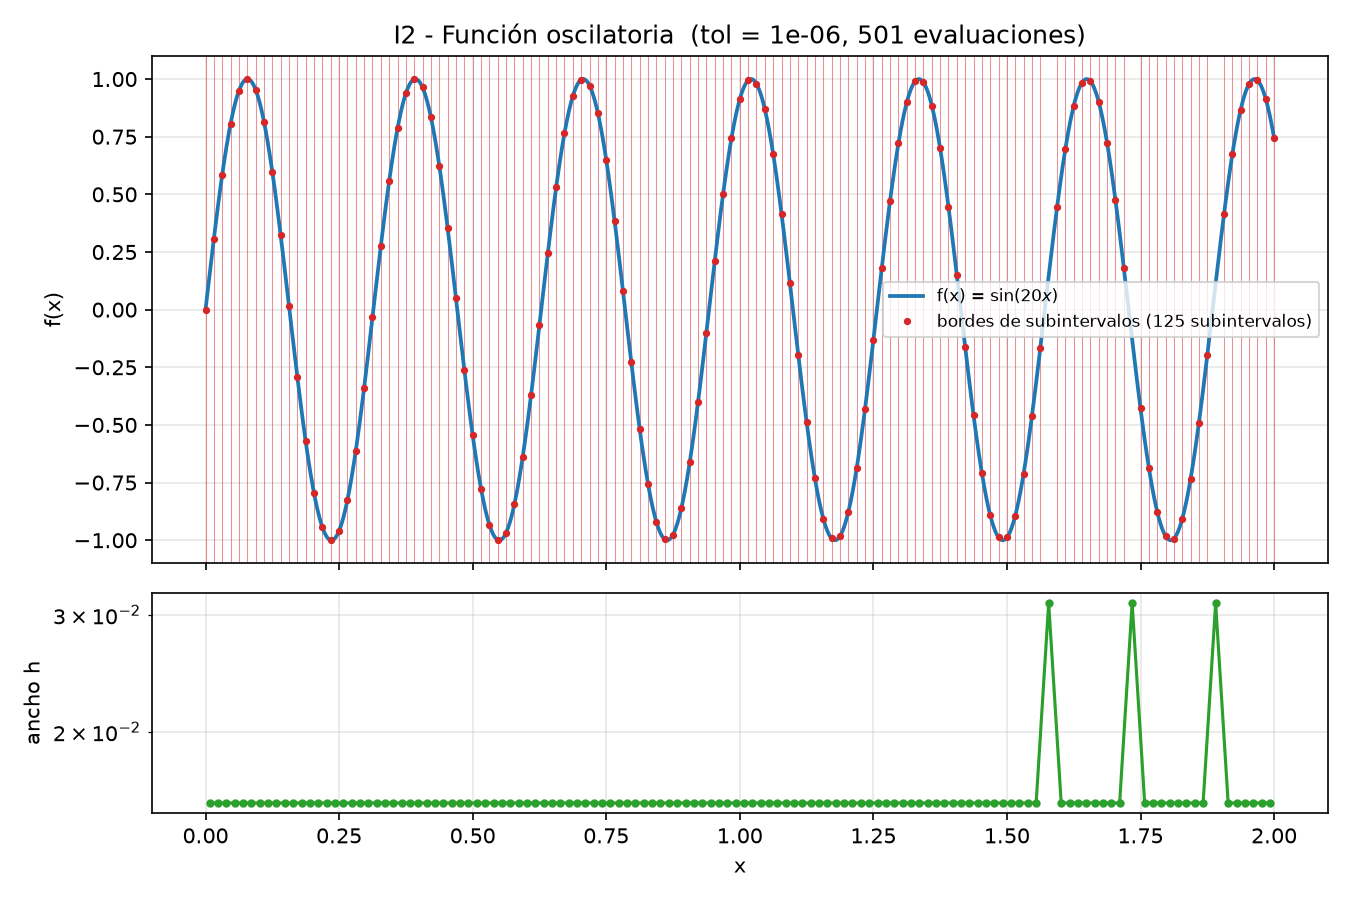
\includegraphics[width=0.85\textwidth]{subintervalos_I2.png}
\caption{$I_2$: la oscilación ocupa todo el intervalo, la partición es casi uniforme.}
\label{fig:sub2}
\end{figure}

\begin{figure}[H]
\centering
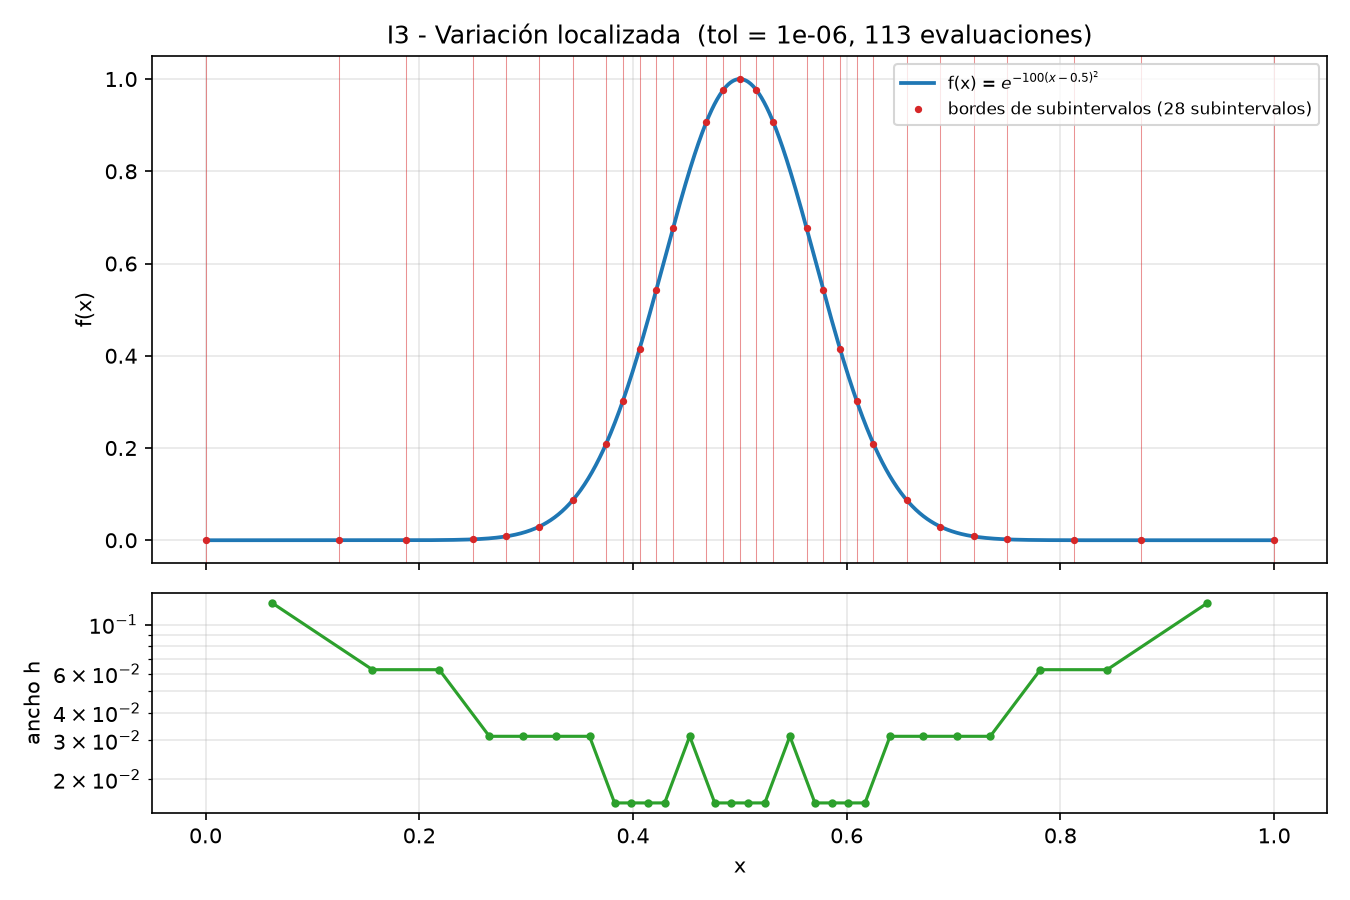
\includegraphics[width=0.85\textwidth]{subintervalos_I3.png}
\caption{$I_3$: los subintervalos se concentran en la campana alrededor de $x=0.5$.}
\label{fig:sub3}
\end{figure}

\begin{figure}[H]
\centering
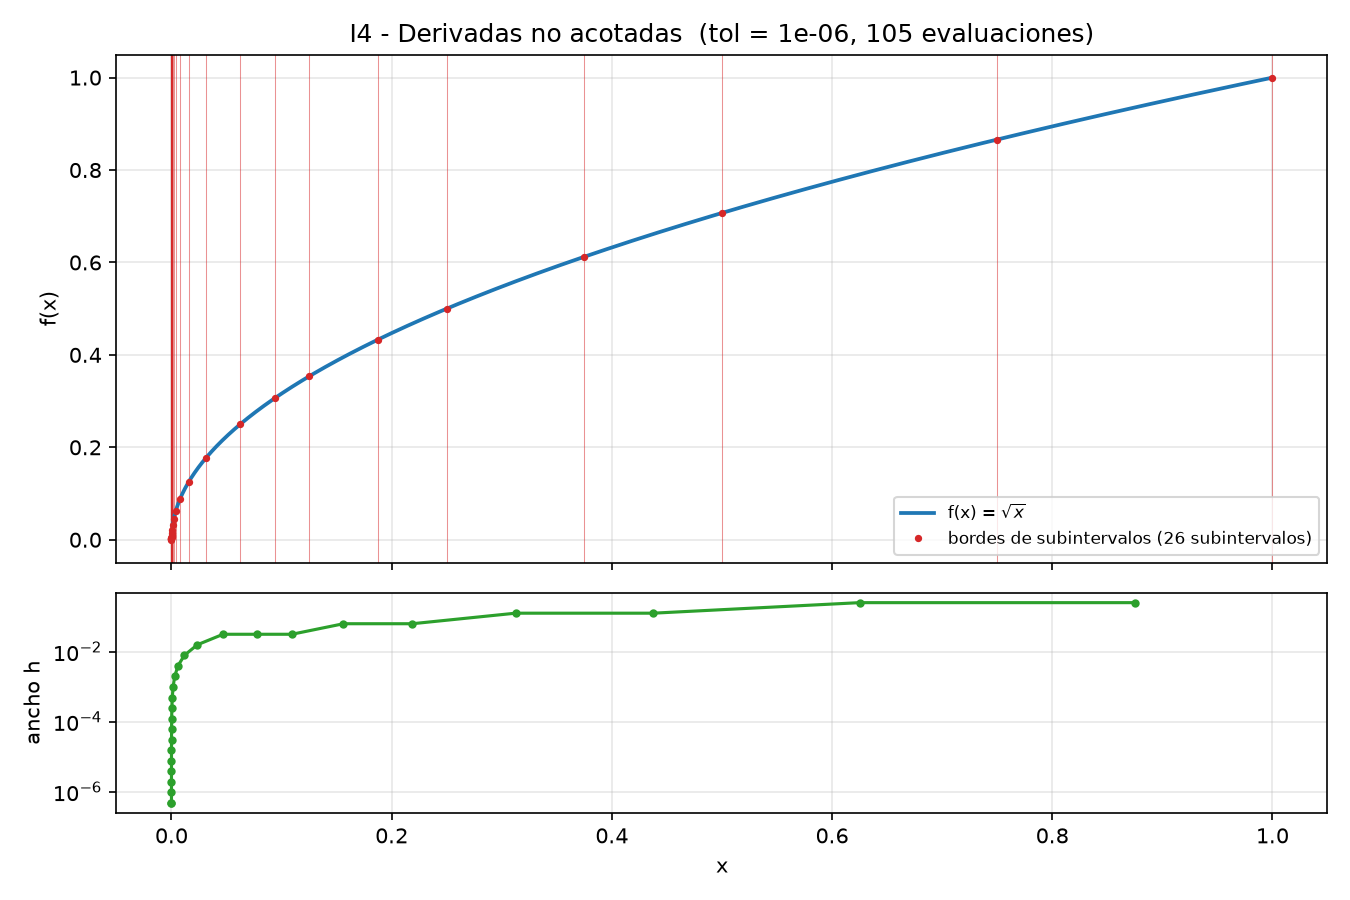
\includegraphics[width=0.85\textwidth]{subintervalos_I4.png}
\caption{$I_4$: refinamiento extremo junto a $x=0$ (anchos de hasta $\approx 5\times10^{-7}$).}
\label{fig:sub4}
\end{figure}

% =================================================================
\chapter{Análisis de resultados}
% =================================================================

\section{¿En qué situaciones Simpson adaptativo es más eficiente que Simpson compuesto?}
El adaptativo gana cuando la dificultad de la función \textbf{no es uniforme} en el intervalo:
\begin{itemize}
  \item \textbf{$I_4=\int_0^1\sqrt{x}\,dx$:} es el caso más claro. Como $f^{(4)}$ no está acotada
        en $x=0$, Simpson compuesto pierde su orden $\mathcal{O}(h^4)$ y sólo converge como
        $\mathcal{O}(h^{1.5})$ (la pendiente de la recta azul en la Figura~\ref{fig:eficiencia}).
        Para $\varepsilon=10^{-6}$ el adaptativo logra error $2\times10^{-8}$ con 105 evaluaciones;
        el compuesto necesita \textbf{25\,849} evaluaciones para el mismo error (unas 250 veces más),
        y para $\varepsilon\le10^{-9}$ no lo alcanzó ni con $2^{24}$ subintervalos.
  \item \textbf{$I_0$ (ejemplo de clase):} la función es tranquila en $[0,2.5]$ y oscila
        rápidamente cerca de $x=4$. El adaptativo usa $h=0.25$ en la parte suave y $h\approx0.002$
        cerca de 4; con 417 evaluaciones tiene error $6\times10^{-8}$, mientras que el compuesto
        con las mismas evaluaciones tiene error $1.6\times10^{-3}$ y necesita unas 5\,300 para igualarlo.
  \item \textbf{$I_1$ y $I_2$:} el adaptativo también resultó entre 3 y 8 veces más eficiente, pero
        aquí la ventaja proviene principalmente de la extrapolación de Richardson
        ($S_2+(S_2-S_1)/15$, orden $h^6$), no de la adaptación, ya que la partición es casi uniforme.
\end{itemize}

\paragraph{Cuándo NO conviene.} En $I_3$ (campana gaussiana) Simpson compuesto fue mucho mejor:
con sólo 27 evaluaciones llegó al error de máquina. Esto ocurre porque la función y todas sus
derivadas son prácticamente cero en los extremos; por la fórmula de Euler--Maclaurin los términos
de error del compuesto se cancelan y converge de forma casi exponencial. El adaptativo, que no
\emph{sabe} esto, sigue refinando según su estimación local y converge sólo de forma algebraica.
También para funciones suaves y baratas el compuesto es más sencillo y no tiene el costo extra
de la recursión.

\paragraph{Comparación con \texttt{quad}.} \texttt{scipy.integrate.quad} (QUADPACK, reglas de
Gauss--Kronrod de 21 puntos) fue el más eficiente en todos los casos, normalmente con error cercano
al de máquina y entre 21 y 273 evaluaciones. Es esperable: usa reglas de orden mucho mayor que
Simpson y técnicas de extrapolación para singularidades. Sirve como referencia de lo que se puede
lograr con un método adaptativo de alto orden.

\section{¿Cómo influye la tolerancia solicitada en el error y en el costo computacional?}
\begin{itemize}
  \item \textbf{Error:} en la Figura~\ref{fig:tol} (izquierda) el error real disminuye al reducir la
        tolerancia y, en 40 de los 45 casos, queda \emph{por debajo} de la tolerancia efectiva
        $\max(\varepsilon,\varepsilon|I|)$. Esto se debe a que el error estimado $|S_2-S_1|/15$ es el
        error de $S_2$, pero se devuelve el valor corregido por Richardson, que es todavía más preciso.
        Por ejemplo, para $I_2$ con $\varepsilon=10^{-6}$ el error estimado fue $3\times10^{-7}$ y el real
        $1.6\times10^{-10}$. Los 5 casos en que se superó la tolerancia son $I_3$ con
        $\varepsilon=10^{-2},10^{-3},10^{-5}$, $I_4$ con $\varepsilon=10^{-3}$ e $I_0$ con
        $\varepsilon=10^{-8}$ (por un factor de 1.2); se analizan en la Sección~\ref{sec:dificultades}.
  \item \textbf{Costo:} en la Figura~\ref{fig:tol} (derecha) las evaluaciones crecen
        aproximadamente como una recta en escala log-log. Como el error local de $S_2$ es
        $\mathcal{O}(h^5)$, para reducir la tolerancia 10 veces el número de subintervalos debe aumentar
        en un factor cercano a $10^{1/4}\approx1.8$. En la Tabla~\ref{tab:tolerancias}, al pasar de
        $10^{-6}$ a $10^{-10}$ (factor $10^4$), las evaluaciones de $I_2$ aumentan de 501 a 4021
        (factor 8, muy cercano a $1.8^4\approx10$).
  \item La relación no es perfectamente suave: hay escalones (por ejemplo $I_1$ usa 5 evaluaciones
        para $\varepsilon=10^{-2},10^{-3},10^{-4}$) porque el número de subintervalos sólo puede crecer
        duplicando intervalos.
\end{itemize}

\section{¿Cómo cambia el número de evaluaciones de la función?}
\begin{itemize}
  \item Siempre se cumple \emph{evaluaciones} $=4N+1$, con $N$ el número de subintervalos finales,
        gracias a que cada subdivisión reutiliza 3 de los 5 valores.
  \item Depende fuertemente de la función: con $\varepsilon=10^{-6}$ se requirieron 17 evaluaciones
        para $e^x$, más de 100 para $I_3$ e $I_4$, y alrededor de 400--500 para las funciones
        oscilatorias $I_0$ e $I_2$. Cuanto mayor es $|f^{(4)}|$ (que para $\sin(20x)$ es $20^4=160\,000$),
        más subintervalos se necesitan.
  \item Para $I_4$ el número de evaluaciones crece lentamente con la tolerancia, aunque la
        profundidad crezca mucho: los intervalos extra se agregan casi sólo en la cadena que
        se acerca a $x=0$, en lugar de dividir todo el intervalo.
\end{itemize}

\section{¿Qué dificultades presenta el algoritmo para funciones con comportamientos complicados?}
\label{sec:dificultades}
\begin{enumerate}
  \item \textbf{Falsa convergencia (aceptación prematura).} En $I_3$ con $\varepsilon=10^{-2}$ y
        $10^{-3}$ el algoritmo se detuvo con sólo 9 evaluaciones y un error real de $2.5\times10^{-2}$,
        mucho mayor que el estimado ($9.6\times10^{-4}$). Con tan pocos puntos, $S_1$ y $S_2$
        ``coincidieron'' por casualidad y el pico no fue detectado correctamente. El mismo riesgo
        existe con funciones muy oscilatorias. Una solución sencilla es obligar a una profundidad
        mínima (dividir siempre los primeros niveles) o usar tolerancias más pequeñas.
  \item \textbf{La estimación del error supone $f^{(4)}$ casi constante.} Cuando no lo es
        (por ejemplo $\sqrt{x}$ cerca de 0, o $I_3$ con $\varepsilon=10^{-5}$, donde el error real
        $1.3\times10^{-5}$ superó al estimado $6\times10^{-6}$), la estimación puede subestimar
        el error. Para $I_4$ con $\varepsilon=10^{-3}$ el error estimado fue $4.4\times10^{-4}$, pero el
        real $3.2\times10^{-3}$: en el primer intervalo $[0,0.5]$ el factor $1/16$ de la deducción no
        es válido porque $\sqrt{x}$ no tiene cuarta derivada acotada.
  \item \textbf{Singularidades en las derivadas.} Para $\sqrt{x}$ el algoritmo converge, pero
        requiere profundidades altas (48 niveles para $\varepsilon=10^{-10}$, con subintervalos de
        ancho $2^{-48}\approx3.6\times10^{-15}$). Si la función tuviera una singularidad más fuerte
        (por ejemplo $1/\sqrt{x}$, que además no se puede evaluar en 0), se alcanzaría el límite
        $k_{\max}$; por eso este límite es indispensable.
  \item \textbf{Redondeo.} Para tolerancias muy pequeñas ($<10^{-12}$) la diferencia $S_2-S_1$
        queda dominada por el error de redondeo y el algoritmo puede subdividir inútilmente.
  \item \textbf{Comportamiento ``escalonado'' del error.} En $I_0$ el error se estanca en
        $3.4\times10^{-8}$ entre $\varepsilon=10^{-7}$ y $10^{-8}$ y luego cae bruscamente: el
        error dominante proviene de un subintervalo concreto que sólo se divide cuando la
        tolerancia baja lo suficiente.
\end{enumerate}

\section{¿Cómo influye el comportamiento de la función en la distribución de los subintervalos?}
El algoritmo usa subintervalos pequeños exactamente donde el error local
$\frac{h^5}{90}|f^{(4)}|$ es grande. Para cumplir la tolerancia con un $|f^{(4)}|$ grande, $h$ debe
ser pequeño; donde $f^{(4)}$ es pequeño, se puede usar $h$ grande:
\begin{itemize}
  \item \textbf{$I_0$} (Figura~\ref{fig:sub0}): en $[0,1.5]$ los intervalos miden $0.25$; a medida que la
        frecuencia de oscilación aumenta hacia $x=4$, el ancho baja hasta $\approx0.002$. El panel
        inferior muestra un ancho que decrece de forma escalonada, siguiendo el aumento de
        frecuencia. Una partición uniforme tendría que usar $h=0.002$ en todo $[0,4]$.
  \item \textbf{$I_1$} (Figura~\ref{fig:sub1}): $e^x$ es suave; 4 subintervalos iguales.
  \item \textbf{$I_2$} (Figura~\ref{fig:sub2}): $\sin(20x)$ oscila igual en todo $[0,2]$, así que la
        partición es casi uniforme ($h\approx0.016$). Aquí la adaptación no aporta ventaja y el
        adaptativo se comporta como un compuesto (con Richardson).
  \item \textbf{$I_3$} (Figura~\ref{fig:sub3}): los intervalos más pequeños ($h\approx0.016$) están en los
        flancos de la campana, en $x\approx0.4$ y $x\approx0.6$, donde la curvatura cambia más; en las
        colas, donde $f\approx0$, se usan intervalos de $0.125$.
  \item \textbf{$I_4$} (Figura~\ref{fig:sub4}): el refinamiento es extremo cerca de $x=0$, donde las
        derivadas de $\sqrt{x}$ tienden a infinito. Cada nivel cerca del origen divide sólo el
        primer intervalo, formando una sucesión geométrica de anchos ($h=2^{-k}$), hasta
        $h\approx5\times10^{-7}$; lejos de 0 se usan intervalos de $0.25$.
\end{itemize}

\section{Conclusiones}
\begin{enumerate}
  \item Se implementó desde cero un algoritmo de Simpson adaptativo que estima el error local
        comparando $S_1$ y $S_2$, combina tolerancias absoluta y relativa, limita la profundidad,
        reutiliza evaluaciones (costo $4N+1$) y registra los subintervalos generados.
  \item El control del error funciona en la gran mayoría de los casos: en 40 de 45 experimentos el
        error real quedó por debajo de la tolerancia, gracias a la corrección de Richardson. Los
        fallos ocurren con tolerancias grandes o cuando la hipótesis de $f^{(4)}$ casi constante no se cumple.
  \item La ventaja del método adaptativo es mayor cuando la dificultad está concentrada:
        para $\sqrt{x}$ y para el ejemplo de clase redujo el número de evaluaciones entre 10 y 250
        veces frente a Simpson compuesto para el mismo error.
  \item No es siempre la mejor opción: para la gaussiana ($I_3$) Simpson compuesto fue superior, y
        con tolerancias grandes el algoritmo puede aceptar resultados erróneos (falsa convergencia).
  \item Las gráficas de subintervalos confirman que el algoritmo coloca los puntos donde la función
        cambia más rápido (oscilaciones, picos y singularidades), que es precisamente el objetivo
        de la integración adaptativa.
\end{enumerate}

\end{document}
